\chapter{Prospects on differential \textsl{t}-channel measurements at 13~TeV}

\intro{Prospects on extending the presented measurements in Ch.~\ref{ch:diff13} are discussed. \Acrlong{pp} collision data corresponding to 36~\invfb recored with the \gls{cms} experiment in 2016 are utilized for this study. Potential improvements in the training of \acrlongpl{bdt}, the fitting procedure, and the unfolding are demonstrated. In particular, the measurement of differential cross section at particle level is envisaged for which technical studies of single top quark events have been published in Ref.~\cite{}.}

%##############################################
\section{Event selection and samples}
%##############################################

%##############################################
\section{Validation}
%##############################################

%##############################################
\section{Extended BDT training}
%##############################################

%##############################################
\section{Fiducial studies}
%##############################################
\label{sec:diff13-fiducial-studies}



Figures~\ref{fig:technique-particle-level-muonpt} and~\ref{fig:technique-particle-level-muoneta} show a comparison of the muon $\pt$ and pseudorapidity at reconstruction, particle, and parton level after selecting events with one muon at each level respectively. The top panels demonstrate a high overlap of the events selected at reconstruction level with the ones at particle and parton level. The acceptance rises with the muon momentum from about 40\% to 90\% due to the relative isolation requirement for reconstructed muons. The number of jets is presented in Fig.~\ref{fig:technique-particle-level-njet}. Due to the jet energy scale correction, 


dressed leptons (cone algorithms associates photons to leptons but does not cluster close leptons), tau decays, jet clustering (no neutrinos/leptons), b-tagging,




particle level overlap: tightMu: >99\%, 2jets: 80\%, 2j1t: 70\%


\myfigure[p]{\label{fig:technique-particle-level}Comparison of expected event densities for $1~\invfb$ at $13~\TeV$ after applying the event selection at reconstruction, particle, and parton level respectively:  (a)~muon $\pt$, (b)~muon rapidity, and (c)~number of jets after requiring one isolated and tight muon; (d)~number of b-tagged jets, (e)~$\pt$ and (f)~pseudorapidity of the spectator jet after requiring one isolated, tight muon and two jets where in (e,f) one jet is additionally required to be b-tagged at reconstruction level. Top panels show the common events selected at reconstruction level while the bottom panels display the acceptance.}{
\subfloat[\label{fig:technique-particle-level-muonpt}]{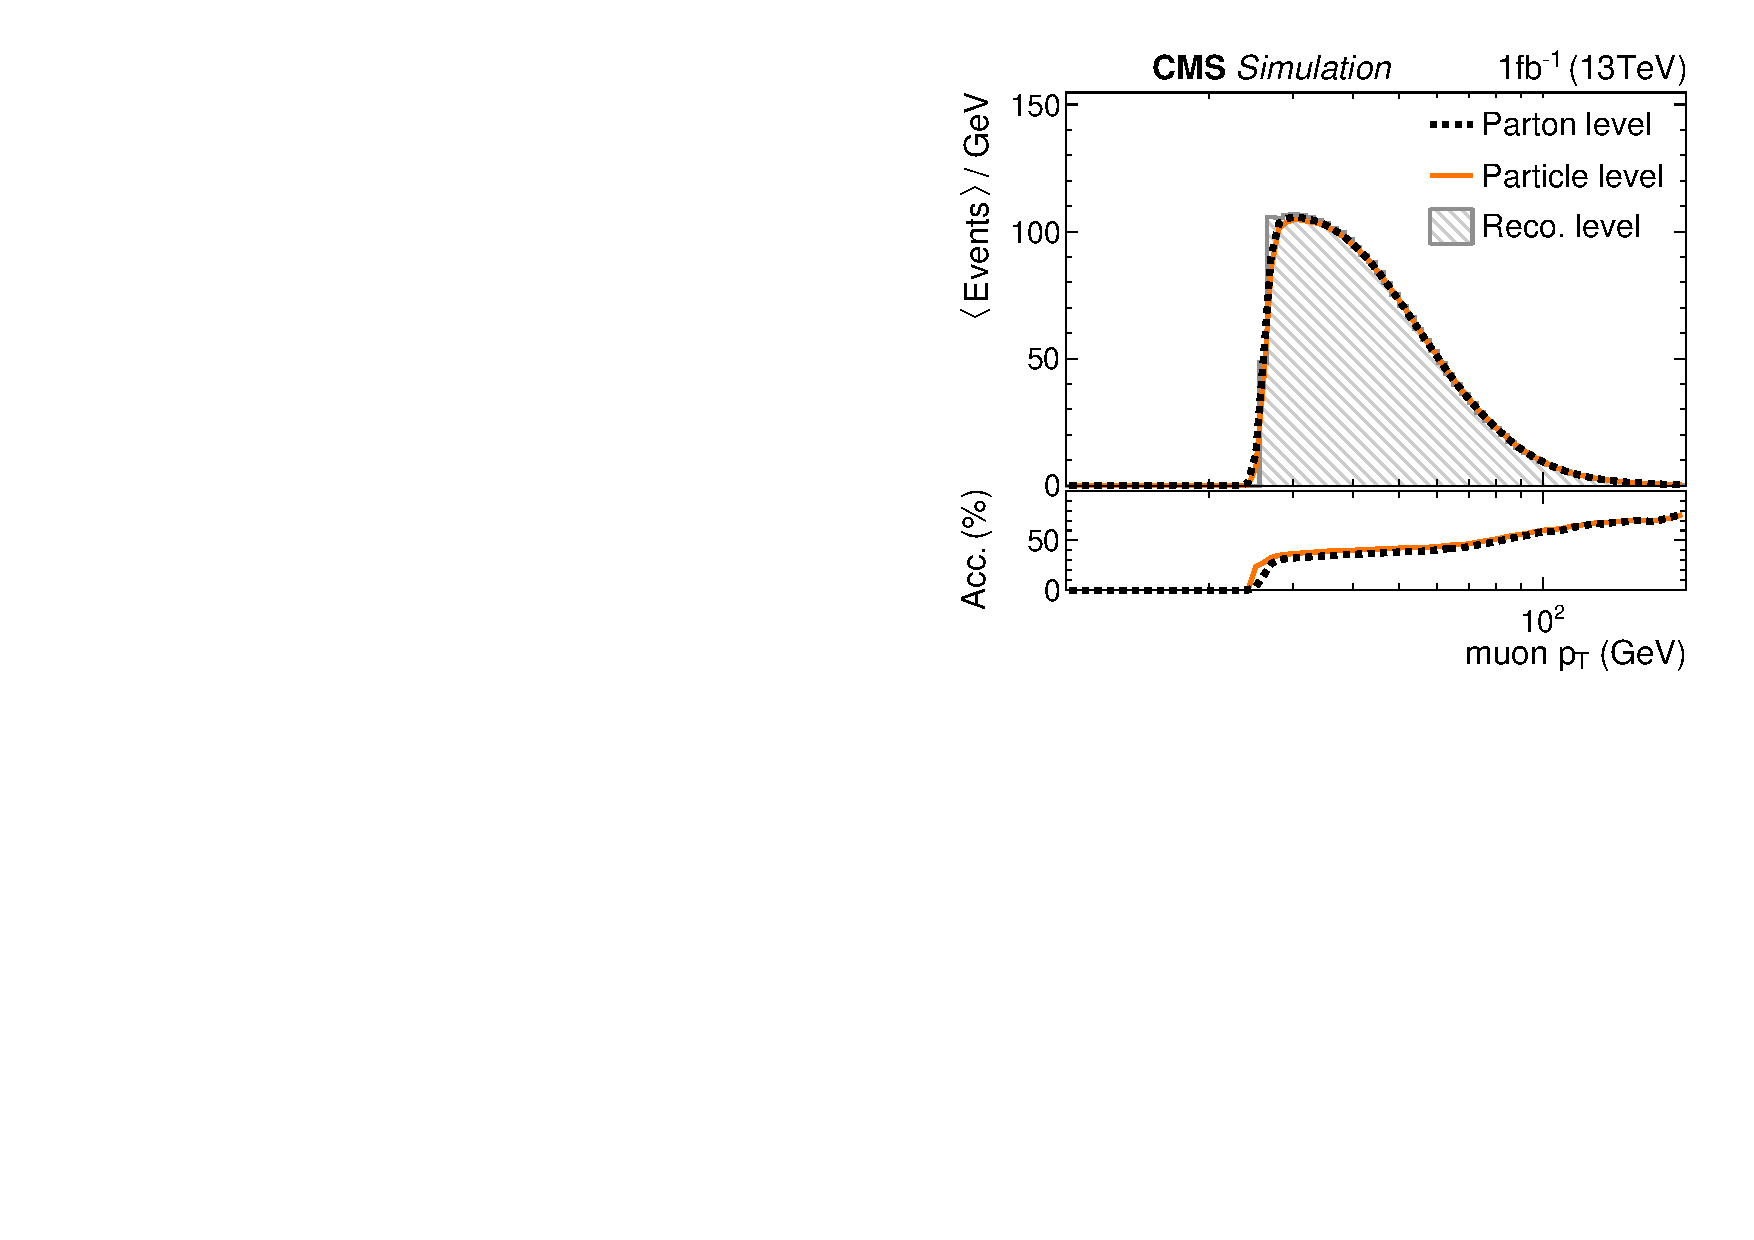
\includegraphics[width=0.48\textwidth]{figures/technique/muon_particle_logpt.pdf}}\hspace{0.03\textwidth}
\subfloat[\label{fig:technique-particle-level-muoneta}]{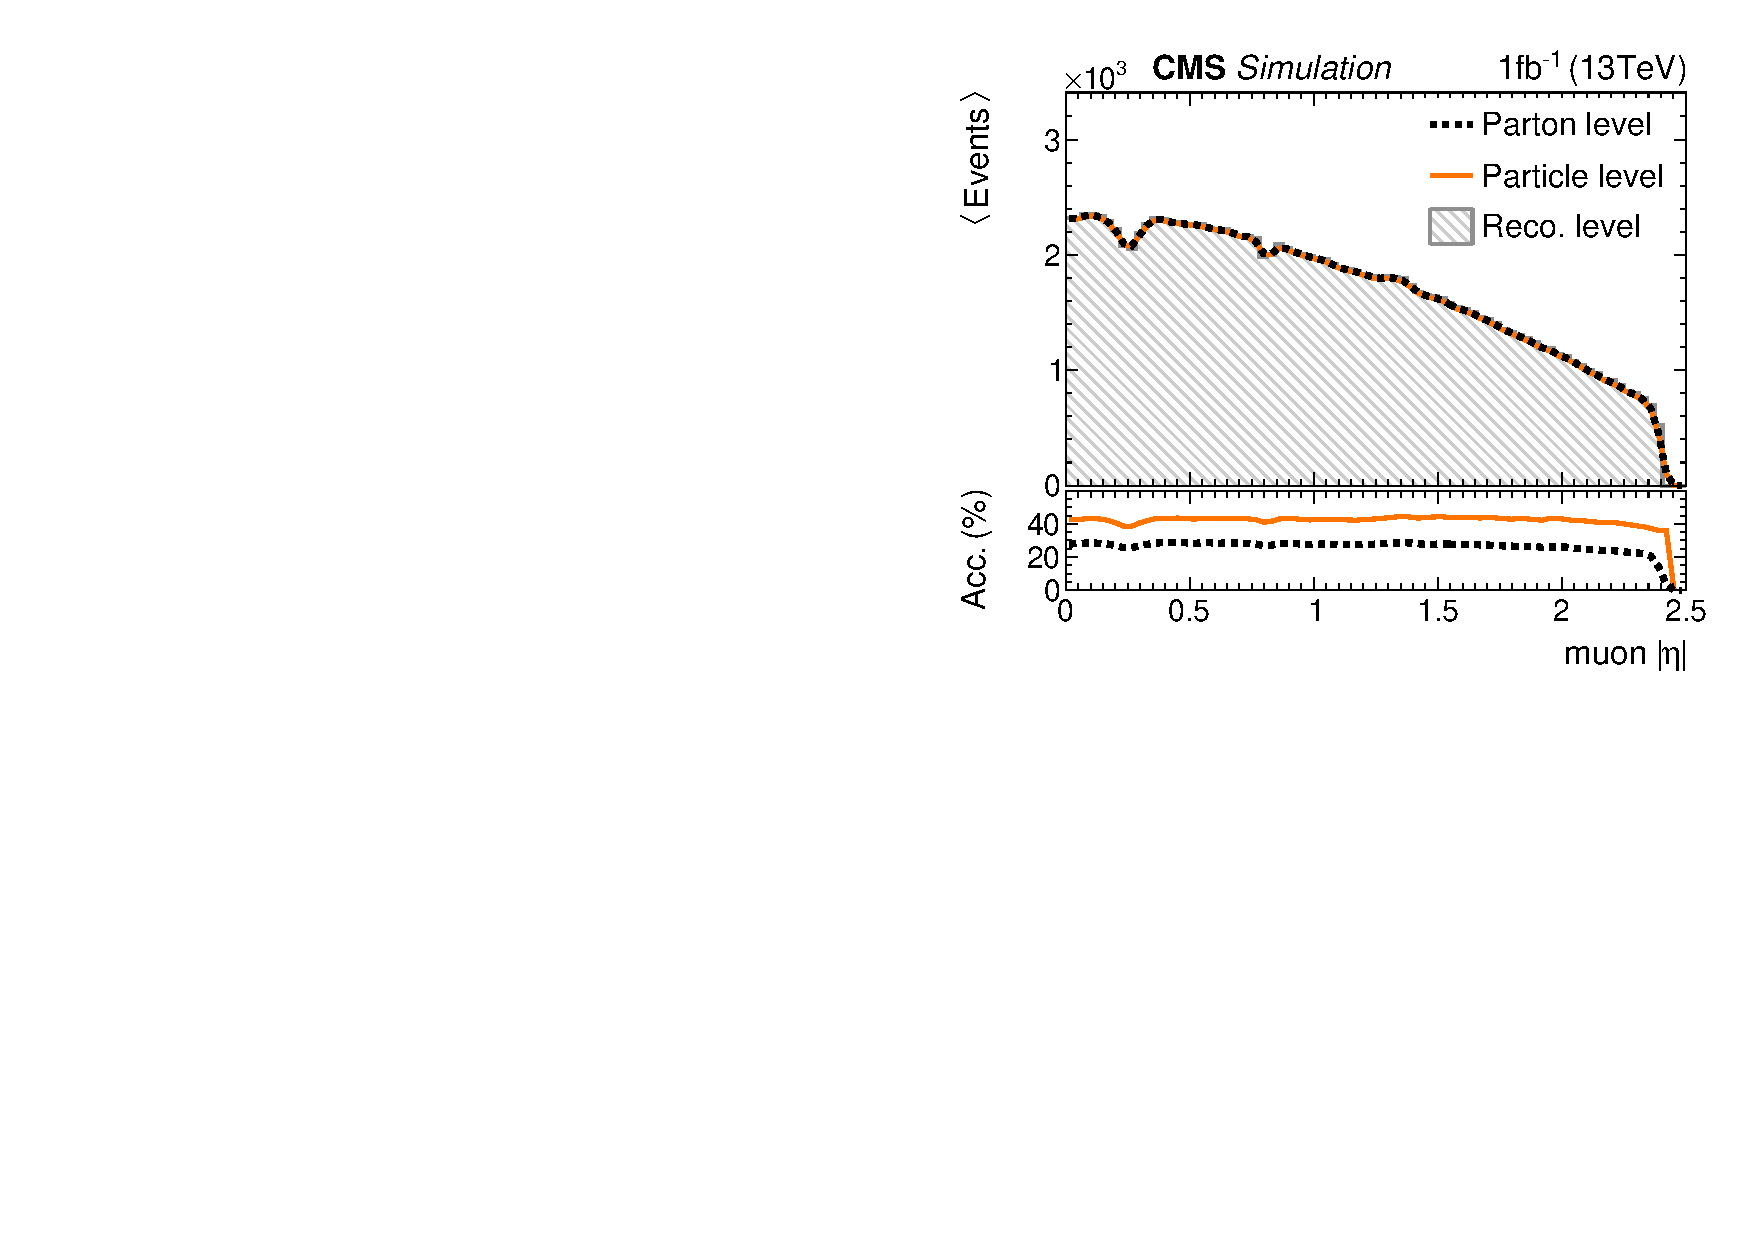
\includegraphics[width=0.48\textwidth]{figures/technique/muon_particle_abseta.pdf}}\\
\subfloat[\label{fig:technique-particle-level-njet}]{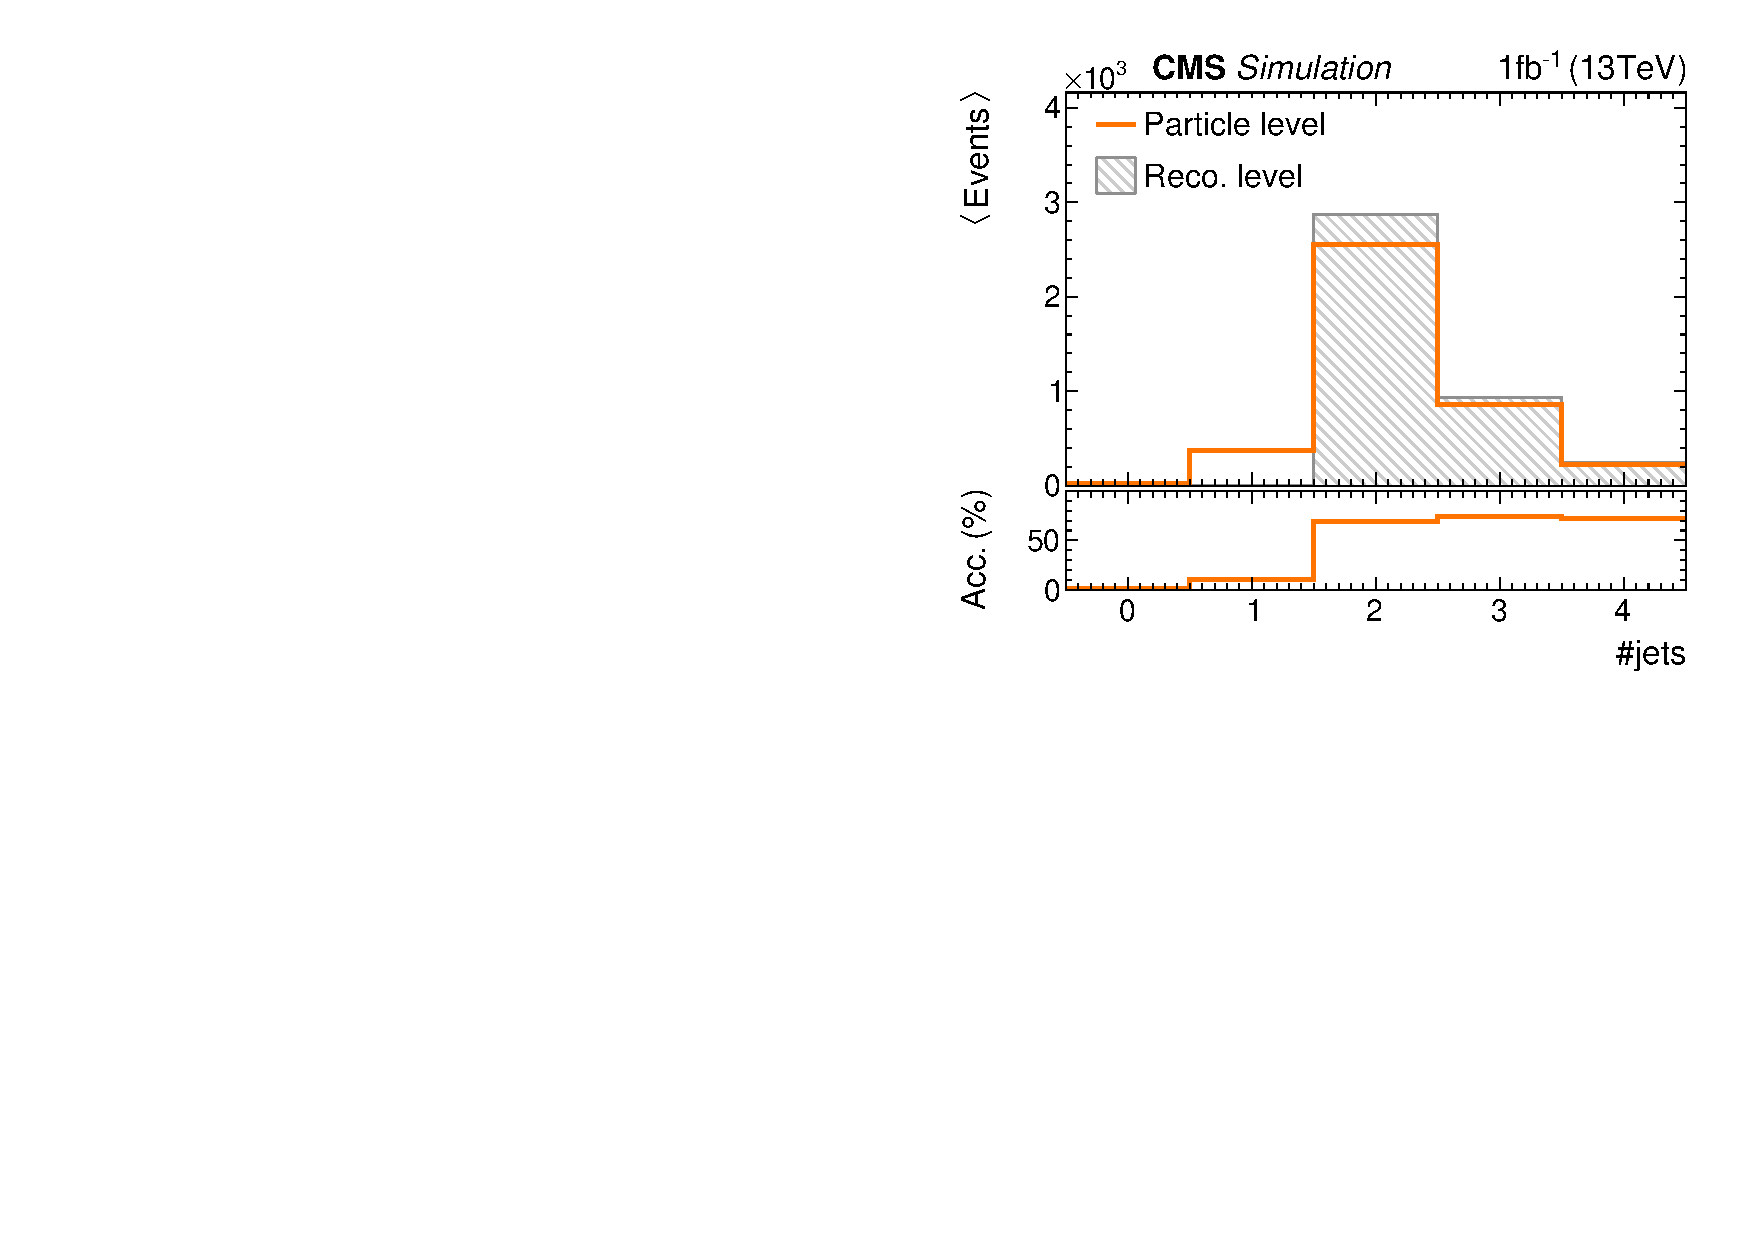
\includegraphics[width=0.48\textwidth]{figures/technique/njet_particle.pdf}}\hspace{0.03\textwidth}
\subfloat[\label{fig:technique-particle-level-nbjet}]{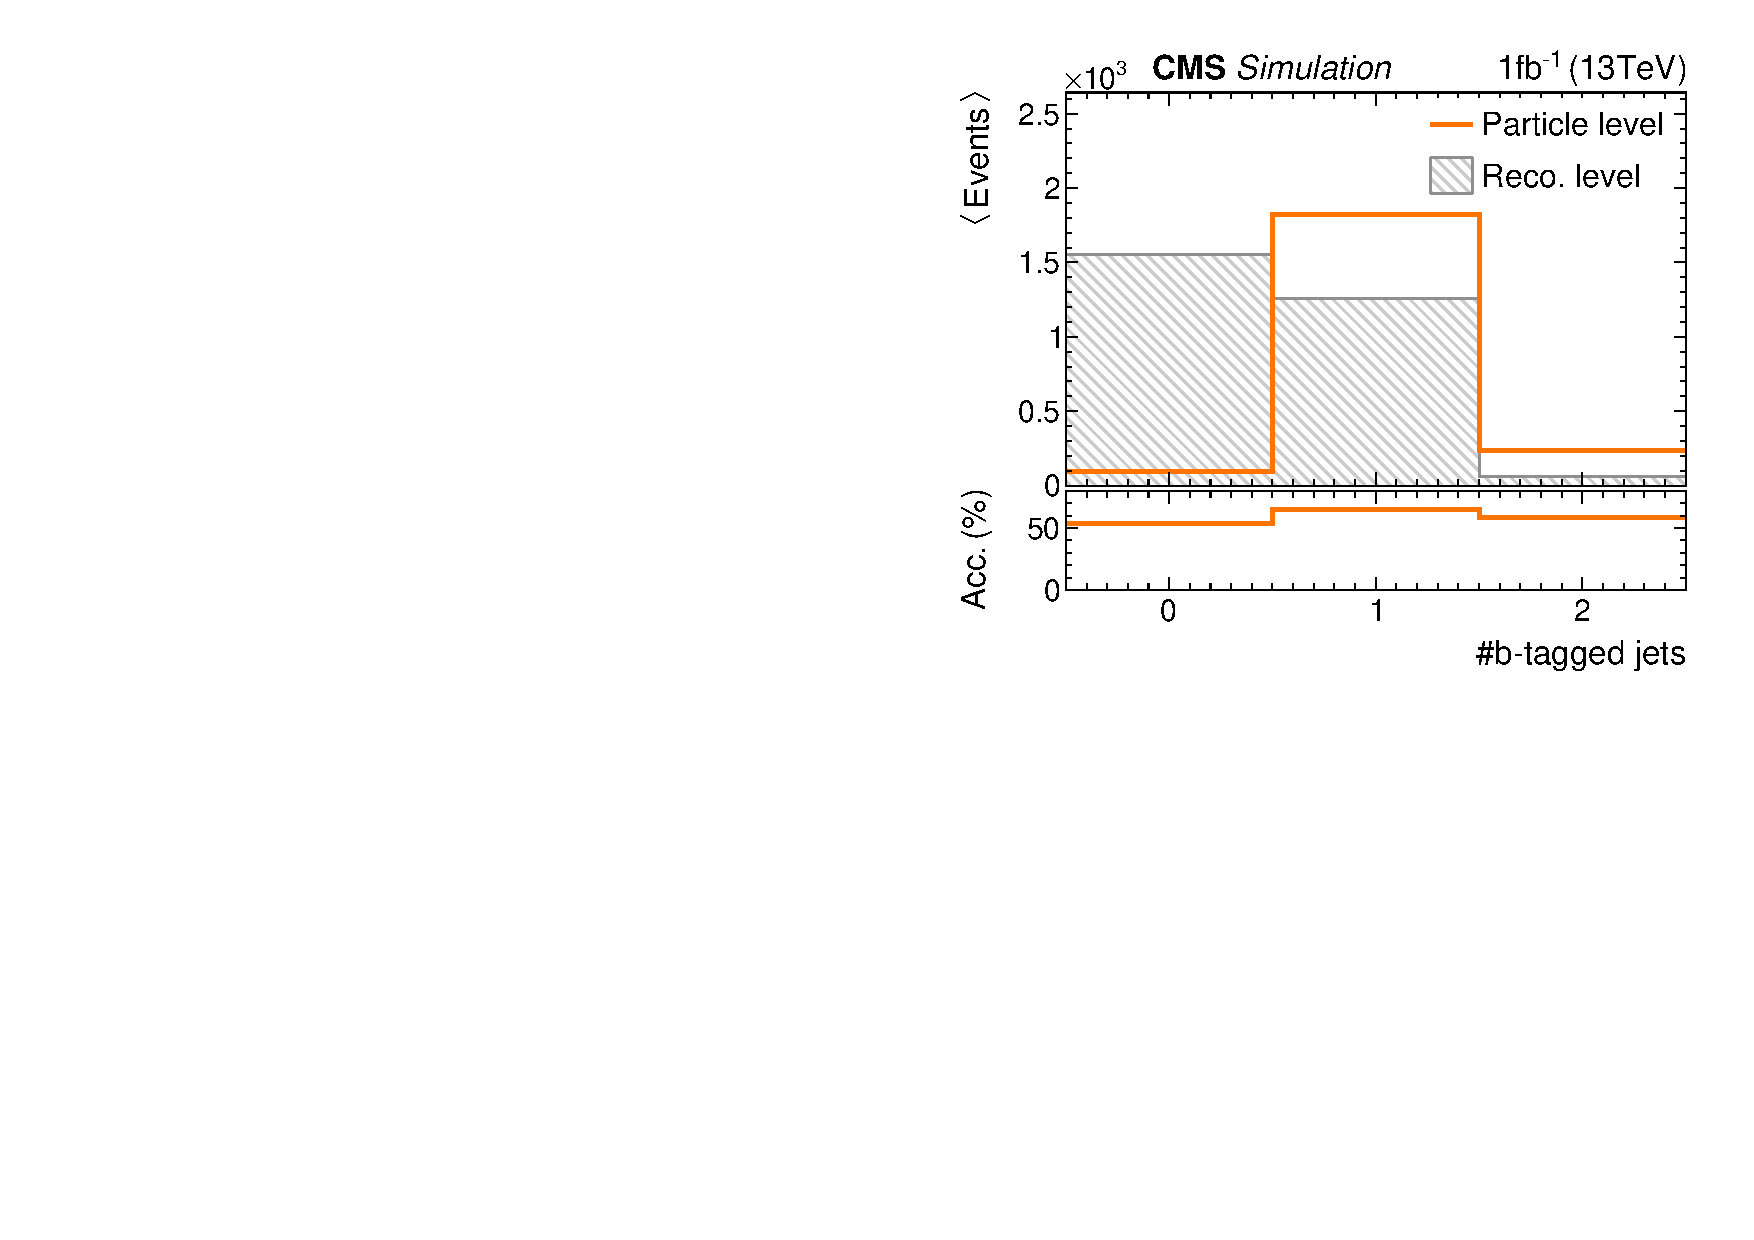
\includegraphics[width=0.48\textwidth]{figures/technique/nbjet_particle.pdf}}\\
\subfloat[\label{fig:technique-particle-level-ljetpt}]{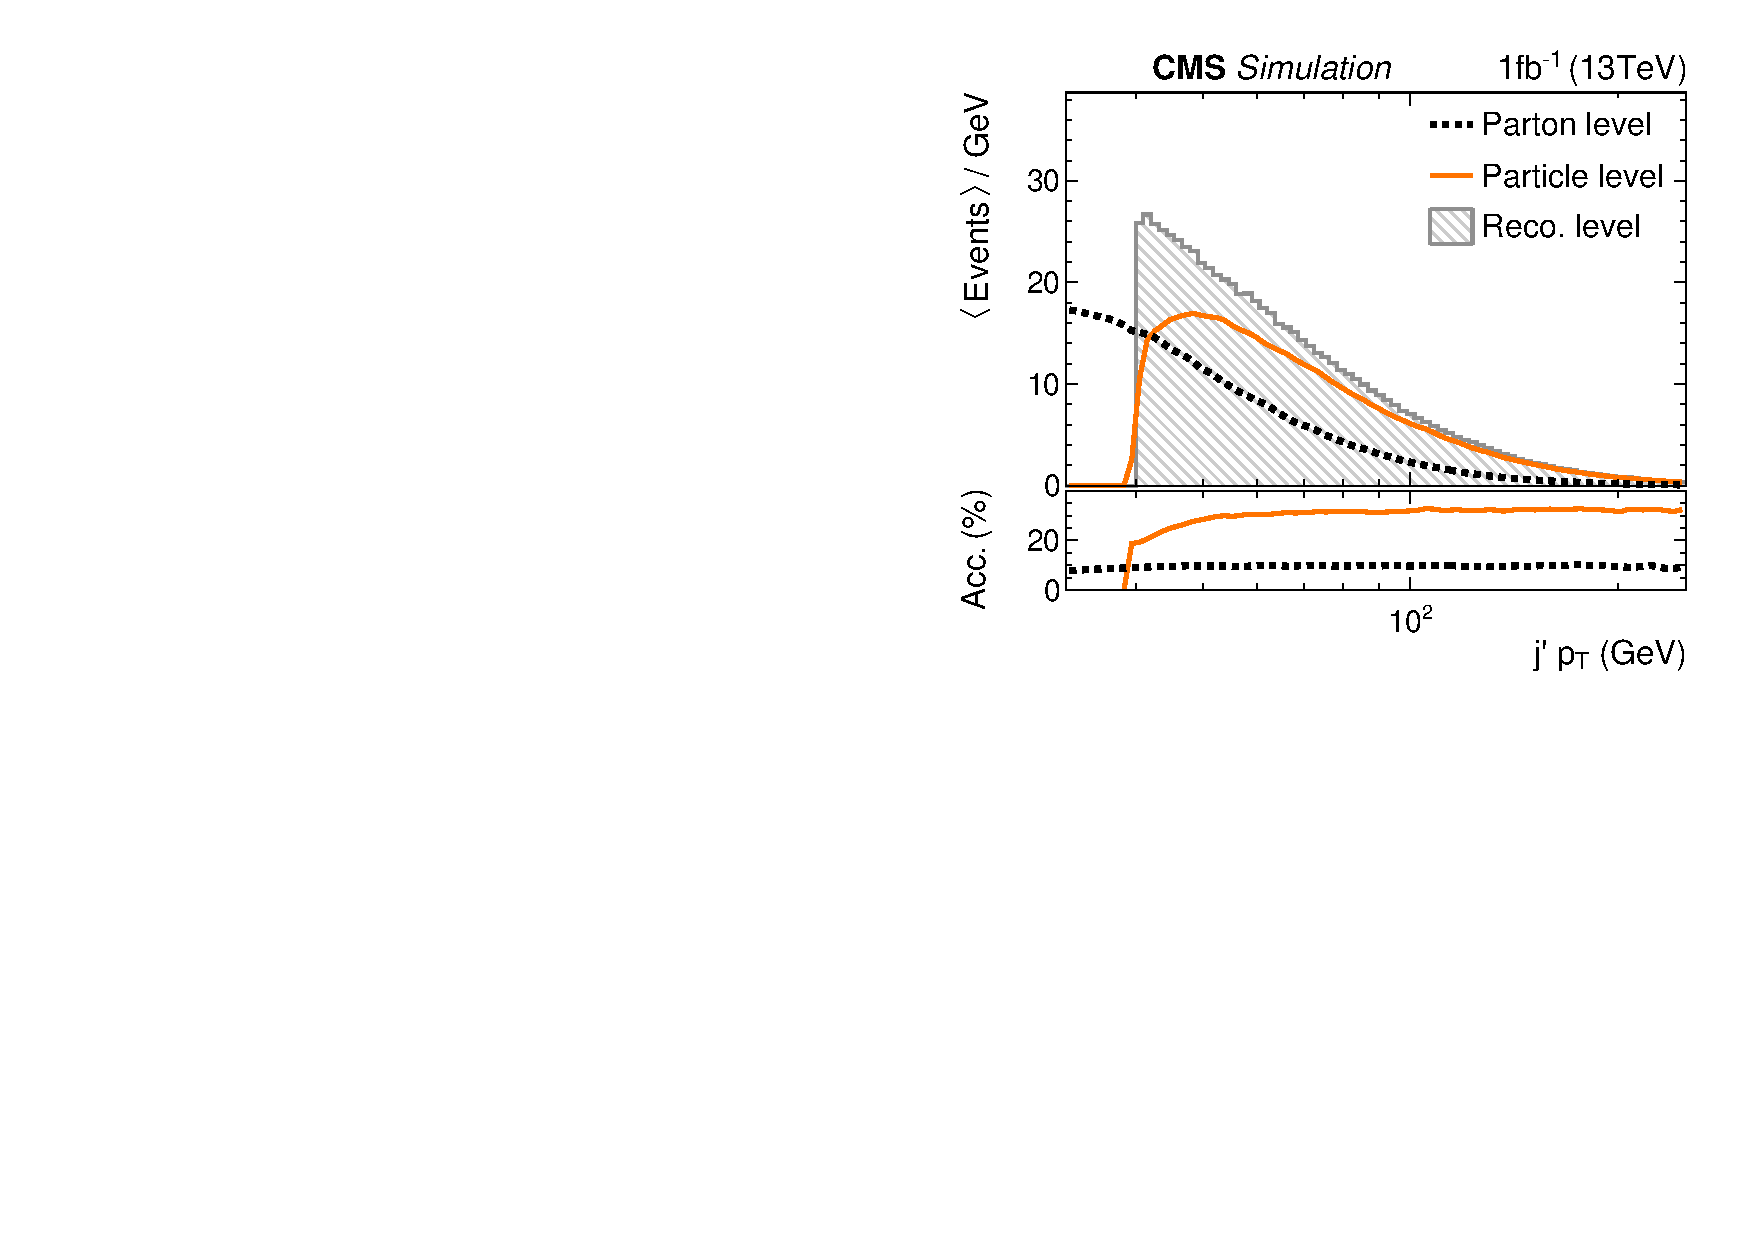
\includegraphics[width=0.48\textwidth]{figures/technique/ljet_particle_logpt.pdf}}\hspace{0.03\textwidth}
\subfloat[\label{fig:technique-particle-level-ljeteta}]{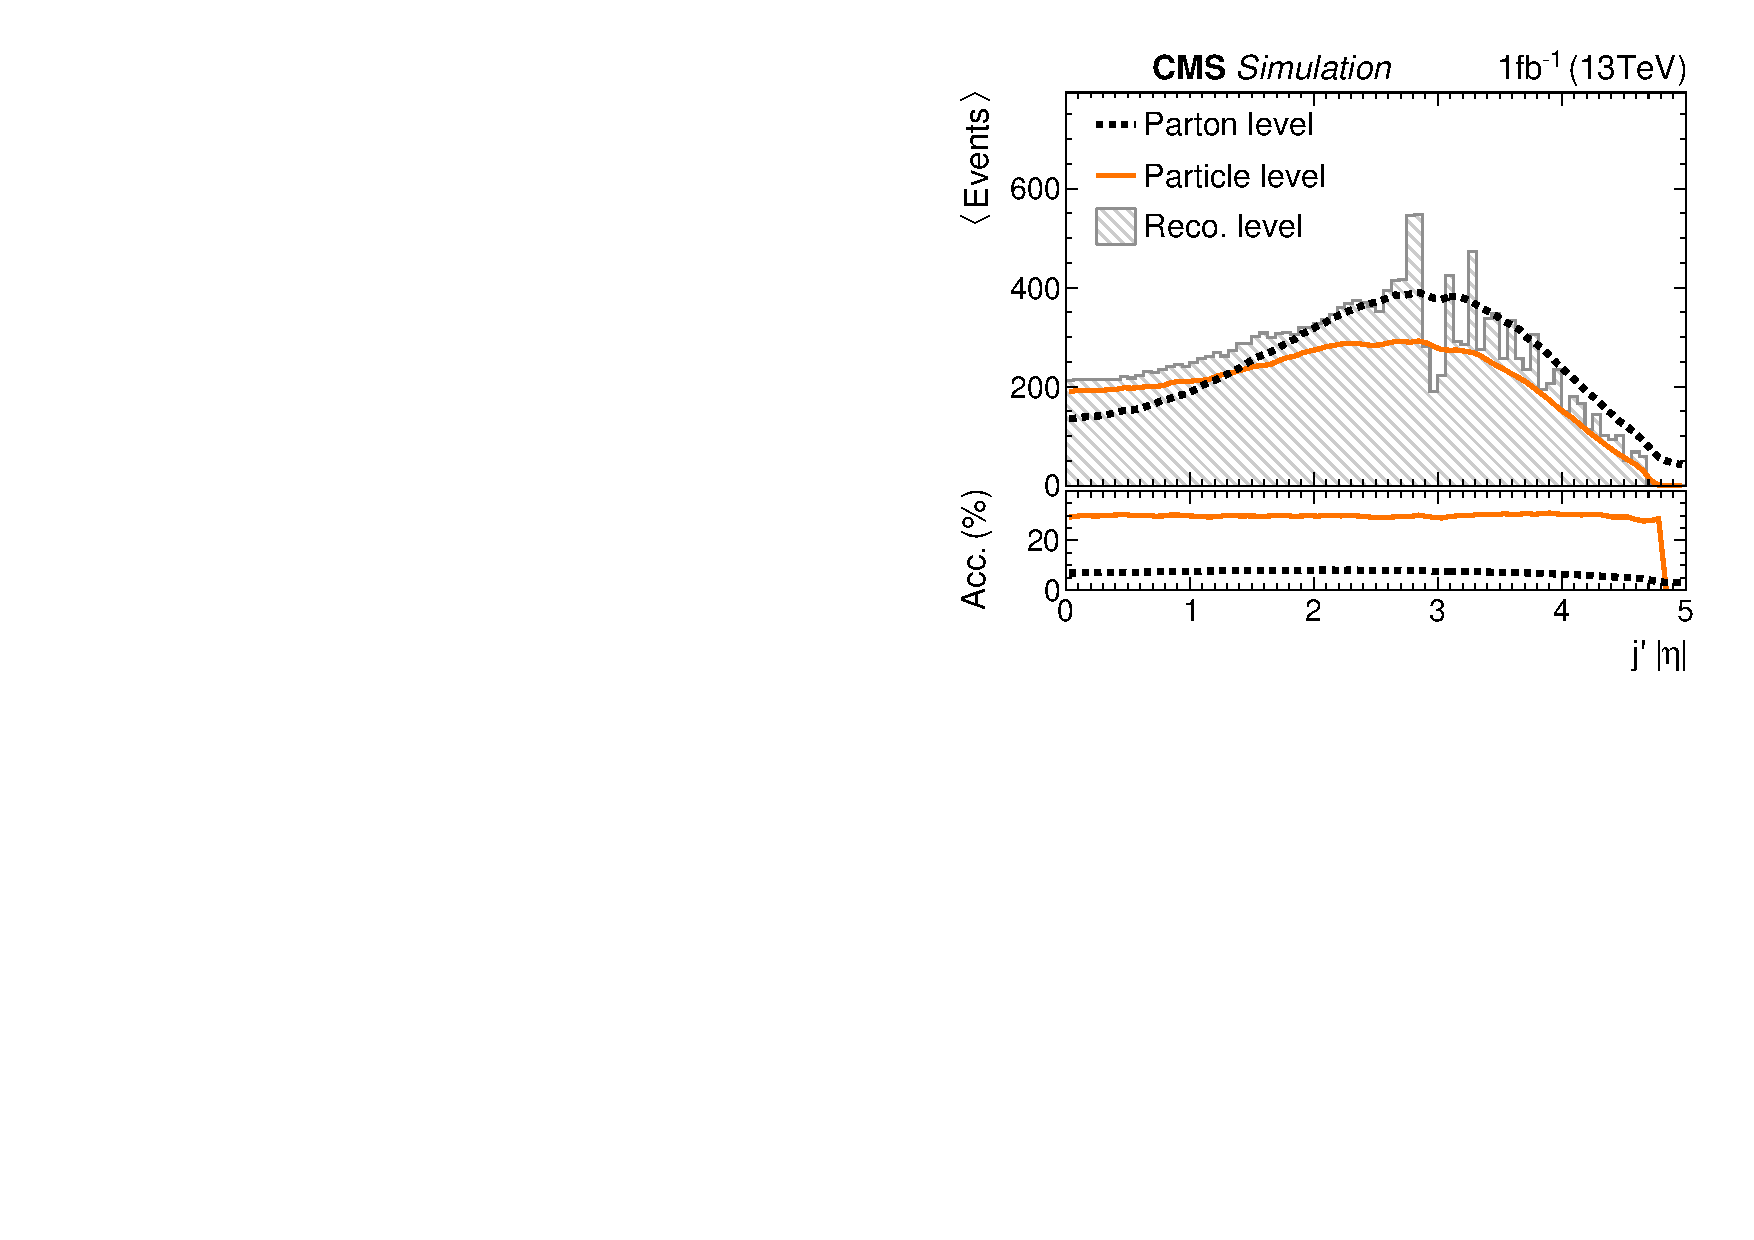
\includegraphics[width=0.48\textwidth]{figures/technique/ljet_particle_eta.pdf}}
}

\myfigure[phtb]{\label{fig:technique-particle-top}Comparison of event selection at reconstruction and particle level.}{
\subfloat[]{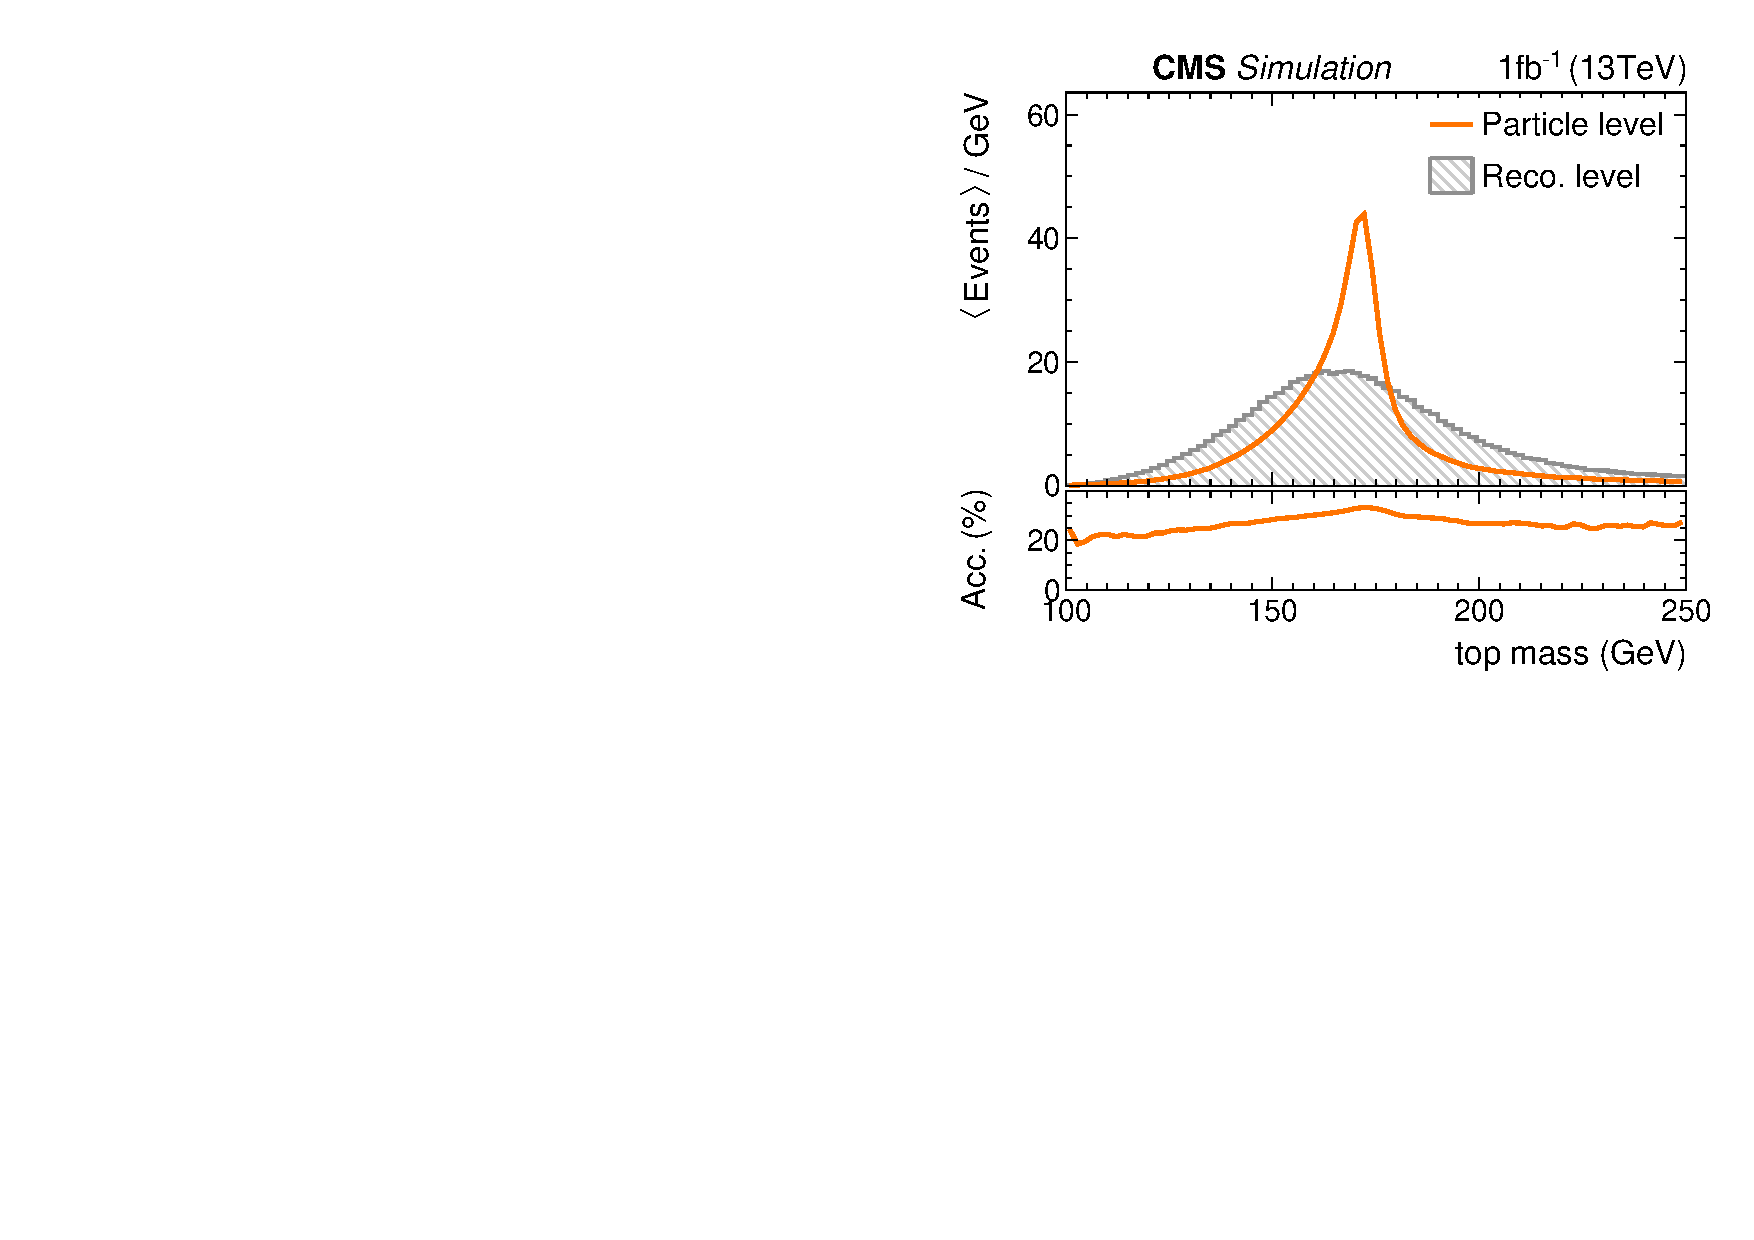
\includegraphics[width=0.48\textwidth]{figures/technique/top_particle_mass.pdf}}\hspace{0.03\textwidth}
\subfloat[]{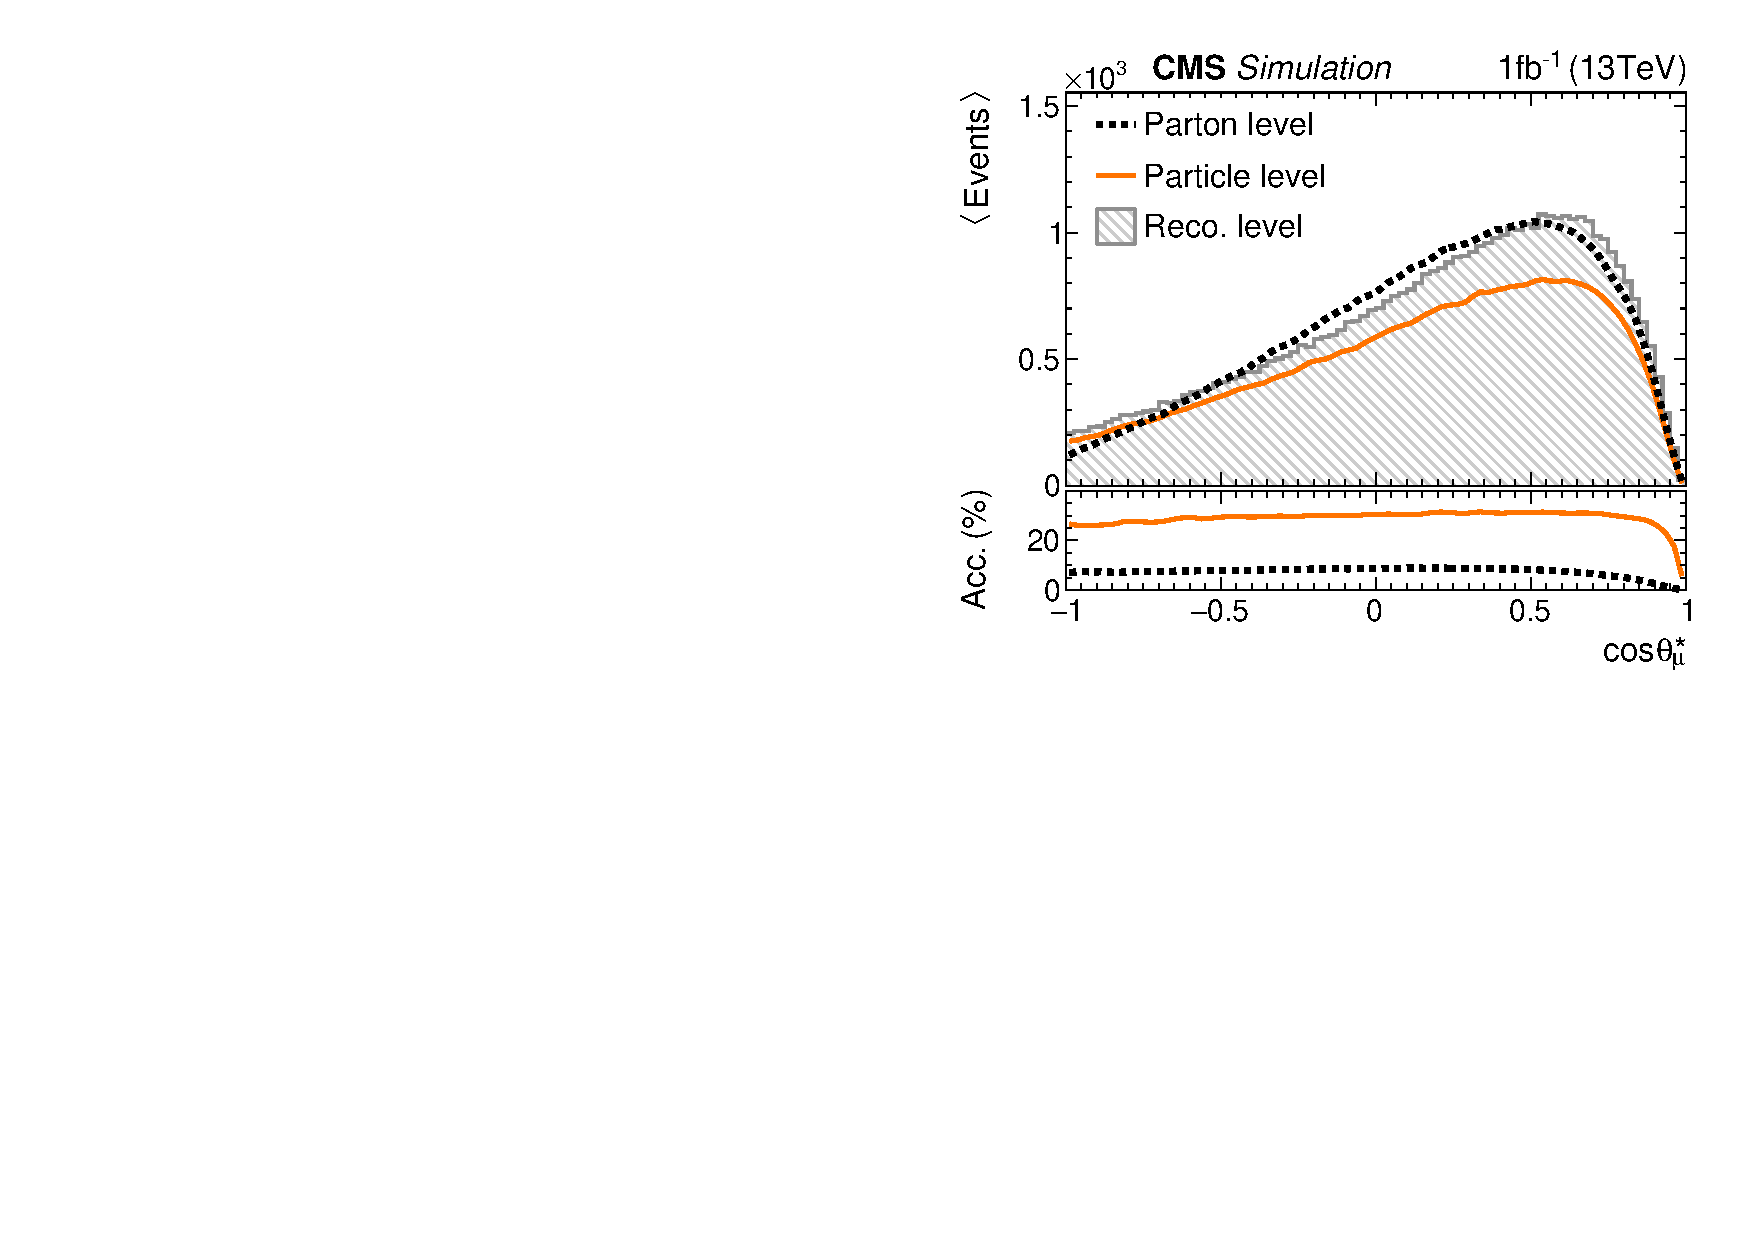
\includegraphics[width=0.48\textwidth]{figures/technique/cosTheta_particle.pdf}}
}

%##############################################
\subsection{Excepted results on pseudo-data}
%##############################################